\section{Findings} \label{findings}
%length: 1 page
%resposible: everybody
%content:

In this section we describe our comparative findings in CS1 and CS3. We start by describing the dropout rates and pass rates in CS1 and CS3. Then we describe the student  performance on the exercised offered in Mumuki per topic. Finally we present our results of applying the Technology Acceptance Model (TAM) to evaluate the acceptance of Mumuki as a tool for supporting learning of Haskell. 

\subsection{Dropout and pass rates}

Tables~\ref{utnCS3} and~\ref{uncCS1} show the dropout and pass rates in CS3 and CS1 during the years 2014, 2015 and 2016. Mumuki was only used during 2016. During 2014 and 2015 the students used directly a compiler (Hugs or Ghci) in order to solve the programming exercises.  

\begin{table}
\begin{tightcenter}
\setlength\tabcolsep{1.9pt}
\begin{tabular}{|l|c|c|c|c|c|c|c|c|c|c|c|c|c|c|c|}

\hline
    & \multicolumn{5}{ |c| }{2014}       
    & \multicolumn{5}{ |c| }{2015}       
    & \multicolumn{5}{ |c| }{2016} \\

\hline
    & S & D & P   & \emph{\%D} & \emph{\%P}  
    & S & D & P   & \emph{\%D} & \emph{\%P} 
    & S & D & P   & \emph{\%D} & \emph{\%P} \\
    
\hline
F	    
    & 7     & 3  & 3   & \emph{43} & \emph{43}	 
    & 6     & 0  & 3   & \emph{0}  & \emph{50}
    & 13    & 1  & 4   & \emph{8}  & \emph{31} \\

\hline    
M	    
    & 44    & 10 & 16   & \emph{23} & \emph{36} 
    & 40	& 13 & 12   & \emph{33} & \emph{30}  
    & 46    & 7  & 18   & \emph{15} & \emph{39} \\
    
\hline
n	    
    & 51    & 13  & 19 & \emph{\textbf{25}} & \emph{\textbf{37}}  
    & 46	& 13  & 15 & \emph{\textbf{28}} & \emph{\textbf{33}} 
    & 59    & 8   & 22 & \emph{\textbf{14*}} & \emph{\textbf{37}} \\

\hline
\end{tabular}
\end{tightcenter}
\caption{Dropout (\%D) and passed rates (\%P) in CS3 at UTN in 2014, 2015 and 2016 discriminated by gender. S stands for Started the course, f for female and m for male. Significant differences are marked with *.}
\label{utnCS3}
\end{table}

Table~\ref{utnCS3} shows that use of Mumuki seems not to have an impact on the pass rate. The pass rate in 2016 is 37\% which is not significantly different of the rates in 2015 (33\%) and 2014 (37\%). We performed a Pearson correlation analysis of each student performance in Mumuki versus his mark in the final test and no correlation was found. However, a significant decrease in the dropout rate can be observed the year Mumuki was used. The dropout rate in 2016 is 14\% while it was 28\% and 25\% in the previous years.  

\begin{table}
\begin{tightcenter}
\setlength\tabcolsep{1.9pt}
\begin{tabular}{|l|c|c|c|c|c|c|c|c|c|c|c|c|c|c|c|}

\hline
    & \multicolumn{5}{ |c| }{2014}       
    & \multicolumn{5}{ |c| }{2015}       
    & \multicolumn{5}{ |c| }{2016} \\

\hline
    & S & D & P   & \emph{\%D} & \emph{\%P}  
    & S & D & P   & \emph{\%D} & \emph{\%P} 
    & S & D & P   & \emph{\%D} & \emph{\%P} \\
    
\hline
F	    
    & 12    & 9  &  2   & \emph{75}  & \emph{17}	 
    & 17    & 10 &  4  & \emph{59}  & \emph{24}
    & 12    & 3  &  7  & \emph{25}  & \emph{58} \\

\hline    
M	    
    & 54    & 29 & 19   & \emph{54} & \emph{35} 
    & 41	& 24 & 14   & \emph{59} & \emph{34}  
    & 43    & 16 & 14   & \emph{37} & \emph{33} \\
    
\hline
n	    
    & 66    & 38  & 21 & \emph{\textbf{58}} & \emph{\textbf{32}}  
    & 58    & 34  & 18 & \emph{\textbf{59}} & \emph{\textbf{31}} 
    & 55    & 19  & 21 & \emph{\textbf{35*}} & \emph{\textbf{38}} \\
    
%\hline
%\emph{\%Female} 
%    & \emph{22\%}   & \emph{23\%}   &   
%    & \emph{13\%}	& \emph{18\%}   &   
%    & \emph{14\%}   & \emph{10\%}   &  \\

\hline
\end{tabular}
\end{tightcenter}
\caption{Dropout (\%D) and passed rates (\%P) in CS1 at UNC in 2014, 2015 and 2016 discriminated by gender. S stands for Started the course, f for female and m for male. Significant differences are marked with *.}
\label{uncCS1}
\end{table}

Table~\ref{uncCS1} shows dropout and passed rates for the CS1 students at UNC. Again Mumuki does not have an impact on the pass rate and no correlation is found between student performance in Mumuki and their mark in the exam. However, an important decrease in dropout rate can be observed the year Mumuki was used. The dropout rate in 2016 is 38\% while it was 59\% and 58\% in the previous years.  

These results are consistent with previous work~\cite{Kumar:2008} on imperative and object oriented languages. Kumar claims that online coding tools similar to Mumuki can be used to improve the retention of students in Computer Science. This is particularly useful in the first CS courses when student's self-confidence is lower. Kumar also claims that the impact is stronger on female students. Our results are not conclusive in this respect probably because of the small percentage of female students. 

The dropout rate in our observational study is high when comparing it to the one in other countries reported in previous work with an
average of 15\% ~\cite{Watson:2014}. Probable causes could be among the following. Both UNC and UTN are public universities and hence they are completely free. Some students work during their studies and others have weak backgrounds in mathematics and need more time to catch up. In general, students that dropout in CS1 quit studying CS. However, students that do not dropout and fail the exam (considered in
the tables) get multiple chances to take it again.    

\subsection{Performance per topic}

We  analyse  student  performance on the different programming topics covered in our course  discriminated  by course level.   Moreover,  we  discuss  common errors in students learning functional programming in our courses. 

We extracted this information automatically from the the system logs. They contain almost 20000 submissions for CS1 with an average of approximately 8 submissions per exercise per student. They contain almost 16000 submissions for CS3 with an average of approximately 5 submissions per exercise per student.  

Figure~\ref{fig:success-rate-by-course} summarises the results of the exercises that the students completed in Mumuki. It indicates the average percentage of exercises assessed in green by Mumuki. The results are presented discriminated by background (CS1 vs CS3). The topics are function composition (including modularity, parameters and simple types), conditionals and boolean operators, pattern matching and tuples, lists and recursion as a basic iterative control structure. 

From the figure we can observe that the CS1 students performance decreases when they start with pattern matching. Observing Mumuki logs and the lecture observations we see one frequent error in this topic. Students do not realise that the order in which they write the patterns may matter. Take for instance the following example. 

\begin{figure}
    \centering
    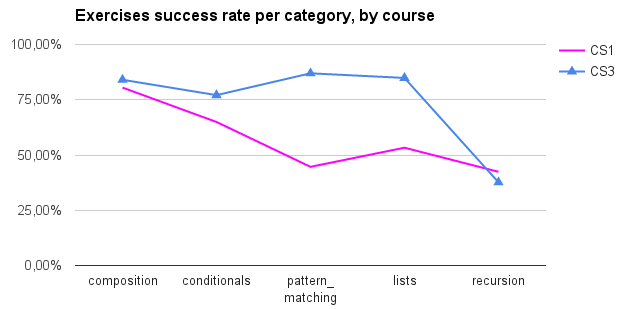
\includegraphics[width=0.4\textwidth]{graphics/success-rate-per-category-by-course.png}
    \caption{Percentage of green exercises per CS group and topic. The topics include function composition, conditionals, pattern matching, lists and recursion.}
    \label{fig:success-rate-by-course}
\end{figure}

\begin{minted}{haskell}
  count0 :: (Show a) => (Int,Int) -> String
  count0 (x,y) = "The pair contains no zero"
  count0 (x,0) = "The pair contains one zero"
  count0 (0,y) = "The pair contains one zero"
  count0 (0,0) = "The pair contains two zeros"
\end{minted}

The last three lines of this program will never be used and the function will always return "The pair contains no zero" even when it contains a zero. This is because all pairs match the pattern (x,y). However, if the order of the lines is inversed the program will work correctly. This error is not common in CS3 probably because of the students' previous experience with imperative programming.

The performance in CS3 decreases in the last topic: recursion. It could be argued that recursion is the control structure that differs the most to the ones learned in imperative programming. A common error is to enter an infinite loop as illustrated in the following example.  

\begin{minted}{haskell}
  delete :: a -> [a] -> [a]
  delete n [] = []
  delete n (x:xs) | n == x = delete n xs
                  | otherwise = delete n (x:xs)
\end{minted}


\subsection{Usefulness and ease of use}

Finally we analyse whether CS1 and CS3 students perceive the usefulness and ease of use differently. To this goal we applied the Technology Acceptance Model (TAM)~\cite{Chuttur:2009}. We performed a survey to all the students that did not dropout (n=87). We asked the students to indicate their level of agreement with the statements listed in Table~\ref{tam-ease-of-use} using a 7-point Likert scale (from 1 to 7). We also asked students to provide free text comments on the best and the worst features of Mumuki.  

CS3 students rate Mumuki less positively in most questions regarding usefulness (statements 1 to 6). The difference in statement 4 is significant (0.99). CS3 students average value for ``Mumuki offers help when I find a task difficult'' is 4.53. 
%The automatic feedback generated by Mumuki includes the results 
%of the test cases and expectations and the output of the compiler. 
Several students in this group mentioned that the errors reported by Mumuki were not clear. One of them said ``Often when I solved an exercise incorrectly, I did not understand the explanation given by Mumuki''.  

CS1 students find Mumuki harder to use than CS3 students (statements 7 to 12). In particular, the difference in statement 8 is significant (0.68). CS1 students average value for ``It was easy to get Mumuki do what I want it to'' is 4.56. 
In the words of the students ``It was frustrating to get the same error over an over again from the system on different submissions''.

\begin{table*}
\begin{tightcenter}
\begin{tabular}{|l|l|c|c|c|c|}
\hline
Statements evaluated (translation from Spanish)	&	TAM reference	&	Female &	Male &	CS1	&	CS3	\\
\hline
1. Mumuki improves my abilities as a Haskell programmer	&	Improvement	&	6.50	&	6.12	&	6.24	&	6.32	\\
2. Mumuki enables me to organise my learning time	&	Productivity	&	6.25	&	5.53	&	5.76	&	5.55	\\
3. Mumuki helps me solve tasks more quickly	&	Efficiency	&	5.50	&	5.59	&	5.56	&	5.74	\\
4. Mumuki offers help when I find a task difficult	&	Helpfulness &	5.63	&	5.47	&	5.52	&	4.53*	\\
5. Mumuki helps me solve tasks correctly	&	Effectiveness &	5.88	&	5.12	&	5.36	&	5.21	\\
6. Mumuki is useful for learning to program in Haskell	&	Usefulness &	6.00	&	6.24	&	6.16	&	5.82	\\
\hline
7. Learning to use Mumuki was easy for me	&	Familiarity 	&	6.25	&	6.18	&	6.20	&	6.74	\\
8. It is easy to get Mumuki do what I want it to 	&	Manageability 	&	4.63	&	4.53	&	4.56*	&	5.24	\\
9. The interaction with Mumuki is clear and understandable	&	Clarity 	&	5.25	&	5.47	&	5.40	&	6.08	\\
10. The interaction with Mumuki is flexible	&	Flexibility  	&	6.13	&	6.35	&	6.28	&	6.45	\\
11. It was easy for me to become skillful at using Mumuki 	&	Proficiency 	&	5.63	&	6.18	&	6.00	&	6.37	\\
12. I think that Mumuki is easy to use	&	Ease of use	&	6.38	&	6.47	&	6.44	&	6.61	\\
\hline
\end{tabular}
\end{tightcenter}
\caption{Results of applying the Technology Acceptance Model (TAM) indicators to the CS1 and CS3 courses. The first six evaluate usefulness and the other are related to ease of use. The results discriminated by gender are also reported for CS1.}\label{tam-ease-of-use}
\end{table*}

The table also shows the data discriminated by gender. Kumar~\cite{Kumar:2008:Female} found that female students assess software tutors more positively than male students. We found no significative difference between genders.  

Among the positive comments made by the students, the most frequent were related to the immediate feedback and its ubiquity. In the students' words: ``It was possible to learn Haskell at any time and place, from any device''. ``One can immediately verify whether an exercise is correct.''

%\begin{figure}
%    \centering
%    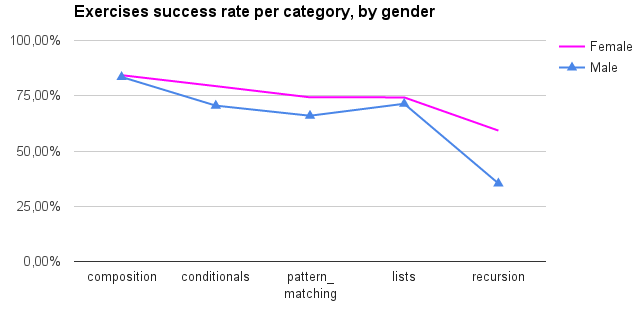
\includegraphics[width=0.4\textwidth]{graphics/success-rate-per-category-by-gender.png}
%    \caption{Caption}
%    \label{fig:success-rate-by-gender}
%\end{figure}

%classify the findings according to some criteria